\documentclass[a4paper, fleqn]{article}
\usepackage{enumitem}
\usepackage{amsmath, amssymb}
\usepackage{xstring}
\usepackage{graphicx} % For including figures
\graphicspath{{./figs/}} % Path to figures
% Set engineering notation
\providecommand{\sci}[1]{\protect\ensuremath{\times 10^{\StrSubstitute[0]{#1}{e}{}}}}
\setlength{\parindent}{0pt} % Set paragraph indentation to zero

\begin{document}

\underline{\textbf{Tutorial 3.1: Fastener}}
\vspace{10pt}

\section*{In-Class activity}
\begin{enumerate}
    \item State the class number of the steel bolts if the proof strength is 315 MPa. \\
    \textbf{Answer:} From table 2.2, select the next higher proof strength (380MPa). Therefore,Class 5.8 is selected.
    \item Determine the preload necessary to be applied on the bolt of class 4.8 with a 6 mm diameter to form a permanent joint.\\
    
    \textbf{Answer:} For permanent joint, use $F_i=0.9F_p$.\\
    where, $F_p=S_p A_t$\\
    From Table 2.2, class 4.8 has $S_p=310MPa$\\
    From Table 2.1, diameter 6mm has $A_t=20.1mm^2=20.1\times 10^{-6}m^2$\\
    Therefore, $F_p=310\times 10^6 \times 20.1\times 10^{-6}=6.23kN$\\
    Finally, $F_i=0.9F_p=0.9\times 6.23=5.61kN$\\
\end{enumerate}

\section*{Theory}

\begin{enumerate}
    \item Proof strength of the steel bolts is obtained from table of specifications and strengths for steel bolts. Explain how to determine the proof strength of the bolt other than steel.
    \item If the external load acting on the bolt is increasing, list ONE (1) improvement that can be done to prevent the joint from separating by assuming the diameter and class number of the bolt areunchanged.
\end{enumerate}


\newpage

\section*{Calculation}
% Note - Need direct question.
\textbf{Question 1}


\begin{figure}[h]
    \centering
    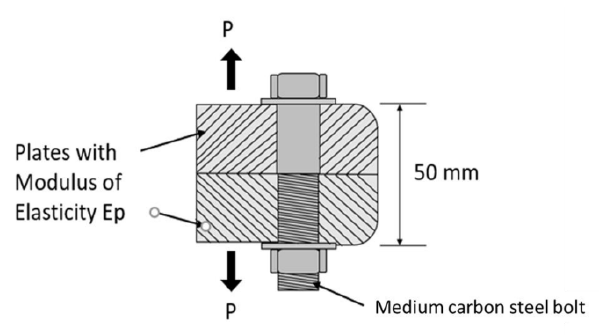
\includegraphics[width=0.5\textwidth]{t31-q1.png}
    \caption{Figure Q1}
\end{figure}

The bolt of connnection M20 x 2.5, ISO coarse thread having Sy = 630 Mpa. The joint carries an external load of P = 40 kN. The bolt were made of steel of modulus elasticity Es and the parts are cast iron with modulus of elasticity Ec = Es/2. Determine

\begin{enumerate}[label=(\roman*)]
    \item The total force on the bolt if the joint is reusable
    \item The tightening torque if the bolts are lubricated
\end{enumerate}

\vspace{10pt}
\textbf{Example Solution}
\vspace{10pt}

$d = 0.02m$\\
$p = 2.5mm$\\
$Sy=630\sci{e6}$Pa\\
$Load,P = 40\sci{e3}$N\\
Engagement length between bolt and nut,\\
$L = 0.06m$\\

i - The total force on the bolt if the joint is reusable

Total force on bolt equation

\begin{equation}
    \begin{aligned}
    F_b=CP+F_i
    \end{aligned}
\end{equation}

where $F_i=0.75F_p$ for reusable joint

First, find joint stiffness factor.
\begin{equation}
    \begin{aligned}
    C=\frac{k_b}{k_b+k_p}
    \end{aligned}
\end{equation}

Find bolt stiffness factor, $k_b$
\begin{equation}
    \begin{aligned}
    k_b=\frac{A_bE_b}{L}
    \end{aligned}
\end{equation}

Change $E_b=E_s$ (steel)

Then, substitue diameter of bolt, d=0.02m and grip distance, L=0.06m to find kb.
\begin{equation*}
    \begin{aligned}
    k_b&=\frac{(\frac{\pi d^2}{4})E_s}{L} \\
    &=\frac{(\frac{\pi 0.02^2}{4})E_s}{0.06} \\
    &= 5.236\sci{e-3}E_s
    \end{aligned}
\end{equation*}

Left $E_s$ as unknown.
\vspace{10pt}

Then, find Part stiffness factor, $k_p$.

\begin{equation}
    \begin{aligned}
    k_p=\frac{0.58\pi E_p d}{2\ln\left( 5\frac{0.58l+0.5d}{0.58l+2.5d} \right)}
    \end{aligned}
\end{equation}

Use $E_p=E_c=\frac{E_s}{2}$

Substitute $E_p=E_s/2$ to kp equation so it can cancel out when finding C in Equation 2.

\begin{equation*}
    \begin{aligned}
        k_p&=\frac{0.58\pi (\frac{E_s}{2}) d}{2\ln\left( 5\frac{0.58l+0.5d}{0.58l+2.5d} \right)}\\
        &=\frac{0.58\pi (\frac{E_s}{2}) (0.02)}{2\ln\left( 5\frac{0.58(0.06)+0.5(0.02)}{0.58(0.06)+2.5(0.02)} \right)}\\
        &= 9.379\sci{e-3}E_s
    \end{aligned}
\end{equation*}


Substitute into joint stiffness factor equation, C (Eq. 2)
\begin{equation*}
    \begin{aligned}
    C&=\frac{k_b}{k_b+k_p} \\
    &=\frac{5.236\sci{e-3}E_s}{5.236\sci{e-3}E_s+9.379\sci{e-3}E_s} \\
    &=\frac{5.236\sci{e-3}}{5.236\sci{e-3}+9.379\sci{e-3}} \\
    &=\frac{5.236}{5.236+9.379} \\
    &=0.3583
    \end{aligned}
\end{equation*}

For reusable joint,$F_i=0.75F_p$ and Proof Strength, $F_p=S_pA_t$.\\
If Yield strength is given, use $S_p=0.9Sy$. \\
Therefore, the Preload equation become,
\begin{equation*}
    \begin{aligned}
        F_i&=0.75F_p\\
        &=0.75(S_pA_t)\\
        &=0.75(0.9S_yA_t)\\
    \end{aligned}
\end{equation*}

$A_t$ is the tensile stress area of the bolt.\\
From Table 2.1, diameter of M20 bolt, $A_t=245\sci{e-6}mm^2$.

Convert to $m^2$.

\begin{equation*}
    \begin{aligned}
        A_t&=245mm^2\\
        &=245mm^2\times(\frac{1m}{1000mm})^2\\
        &=245\times1\sci{e-6}\\
        &=245\sci{e-6}m^2
    \end{aligned}
\end{equation*}

Substitute into Preload equation,
\begin{equation*}
    \begin{aligned}
        &=0.75(0.9S_yA_t)\\
        &=0.75(0.9)(630\sci{e6})(245\sci{e-6})\\
        &=1.042\sci{e5}N
    \end{aligned}
\end{equation*}

Substitute into Total force on bolt equation (Eq. 1)

\begin{equation*}
    \begin{aligned}
        F_b&=CP+F_i\\
        &=0.3583(40\sci{e3})+1.042\sci{e5}\\
        &=1.185\sci{e5}N
    \end{aligned}
\end{equation*}

ii- The tightening torque if the bolts are lubricated

If joint are lubricated, k=0.15
\begin{equation}
    \begin{aligned}
        T&=kdF_i\\
        &=(0.15)(20\sci{e-3})(1.042\sci{e5})\\
        &=312.56N.m
    \end{aligned}
\end{equation}

\newpage
\textbf{Question 2}
% Unknown kp

\begin{figure}[h]
    \centering
    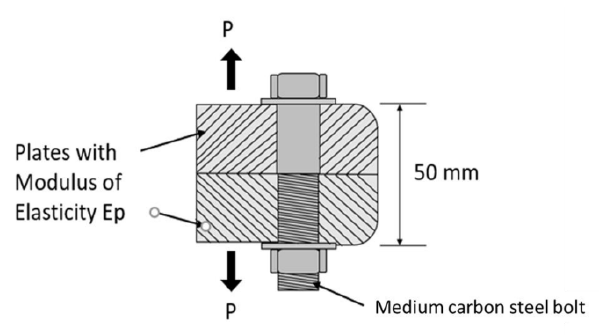
\includegraphics[width=0.5\textwidth]{t31-q2.png}
    \caption{Figure Q1}
\end{figure}

A section of connection illustrated in Figure 1 forms a reusable connection. A total of 4 bolts are used to resist an external load 150 kN. The bolt connection is M14 x 1.5 ISO fine threadclass 5.8, made from medium carbon steel with modulus of elasticity of 200 GPa. The stress in each bolt is 406.2MPa. Determine;

\begin{enumerate}[label=(\roman*)]
    \item The joint stiffness factor.
    \item Stiffness constant for bolt and plates.
    \item Modulus of elasticity of plate Ep
    \item Suggest suitable material used for plates (Based on answer in iii)
\end{enumerate}


\newpage
% Use simple kp
\textbf{Question 3}

\begin{figure}[h]
    \centering
    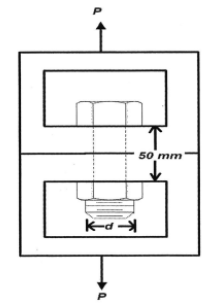
\includegraphics[width=0.5\textwidth]{t31-q3.png}
    \caption{Figure Q3}
\end{figure}

A bolted assembly of two parts is shown in Figure Q3, is to support an external load, P = 80 kN. The steel bolt is fine thread and the modulus of elasticity is 200 GPa and reused connection. The joint stiffness factor for the design is 0.286. The parts are made of cast iron with a modulus of elasticity of 70 GPa. Assume the factor of safety for the joint is 2. Determine;

\begin{enumerate}[label=(\roman*)]
    \item The stiffness constant for the part of the effective area of the part is 2500 $mm^2$
    \item The stiffness constant for the bolt and size of the bolt, d.
    \item The suitable metric specification class number for the bolt.
\end{enumerate}


\newpage
% Well-defined
\textbf{Question 4}

\begin{figure}[h]
    \centering
    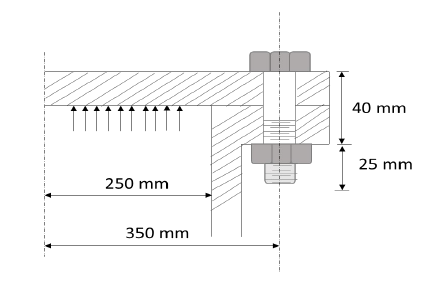
\includegraphics[width=0.5\textwidth]{t31-q4.png}
    \caption{Figure Q4}
\end{figure}

Given M10 x 1.5 grade 5.8 bolts used to create a permanent joint connection for a pressure cylinder. A total of 2 number of bolts of modulus of elasticity 200 GPa is used to carries external load P = 8kN. The joint parts are cast iron ASTM A-48 with modulus of elasticity of 70 GPa. Determine;

\begin{enumerate}[label=(\roman*)]
    \item The stiffness constant for bolts, parts and joint’s stiffness factor
    \item Proof strength of the bolt
    \item Yield strength of the bolt
    \item The preload on the bolt
    \item The forces on the bolt and will the part be separated under load P?
    \item The forces on the part
    \item The torque on the bolt if the joint is lubricated
    \item Pressure of gas on the cylinder if the diameter of the cylinder is 250 mm.

\end{enumerate}

Well-defined problem

1. If the external load is increased by 60\%, suggest improvements need to be done to avoid separation?

2. Recommend the maximum pressure if the number of bolts is increased to 6

3. Is the joint safe or fail if the pressure is increased 30\%. Prove your answer.

4. If the external load is increased by 50\%, suggest the suitable metric specification class number for the bolt.


\newpage

\textbf{Answer}
\vspace{10pt}

\textbf{Q2}

i- The joint stiffness factor, $C=0.404$

ii- Stiffness constant for bolt, $k_b=6.158\sci{e8}N/m$ and plates, $k_p=9.084\sci{e8}N/m$

iii- Modulus of elasticity of plate, $E_p=73.65GPa$

iv- Suggest suitable material used for plates (Based on answer in iii)

Structural steel ASTM A-36, High-strength Steel ASTM A-242

\vspace{10pt}
\textbf{Q3}

i- The stiffness constant for the part of the effective area of the part is $k_p=3.5\sci{e9}$

ii- The stiffness constant for the bolt is $k_b=1.402\sci{e9}N/m$ and size of the bolt, d=24mm

iii- Minimum proof strength for the design is 476.67MPa.
From Table 2.2, the next higher Proof strength is 600MPa. The suitable metric specification class number for the bolt is 8.8.

\vspace{10pt}
\textbf{Q4}


i- The stiffness constant for bolts, $k_b=3.927\sci{e8}N/m$, parts, $k_p=5.941\sci{e8}N/m$ and joint’s stiffness factor, $C=0.3986$

ii- Refer to Table 2.2, Class 5.8 has Proof strength, $S_p=380MPa$

iii- Yield strength of the bolt, $S_y=422.22MPa$

iv- The preload on the bolt, $F_i=1.9836\sci{e4}N$

v- The forces on the bolt, $F_b=21.428kN$ and the part will not be separated under load P.

vi- The forces on the part, $F_p=-17.428kN$

vii- The torque on the bolt if the joint is lubricated, $T=29.754N.m$

viii- Pressure of gas on the cylinder if the diameter of the cylinder is 250 mm, $P_{max}=163kPa$

\vspace{10pt}
Well-defined problem

1. Option 1: Increase the number of bolts to reduce the load on each bolt.
Number of bolts, n = 3

Option 2: Increase size of bolt to increase effective cross-sectional area. \\
The next larger $A_t$ is 84mm. The new bolt size will be M12.

Option 3: Use higher class of bolt. Maintain the same size of bolt and number of bolts. \\
The next higher Proof strength is 600MPa. The suitable metric specification class number for the bolt is 8.8.

2. The maximum pressure if the number of bolts is increased to 6 is $P_{max}=676.9kPa$

3. The joint is safe if the pressure is increased 50\%. \\
New Pressure, $10400Pa$ \\
Total force on bolt, $F_b=21.91kN$ \\
Since, $F_b >P$, the joint is safe.

4. New load, $P_{new}=1.5*8000=12000N$ \\
From Table 2.2, the next higher Proof strength is 600MPa.
The suitable metric specification class number for the bolt is 8.8.

\end{document}